
\section{Supporting Construction Artifacts}

\begin{figure}
    \centering
    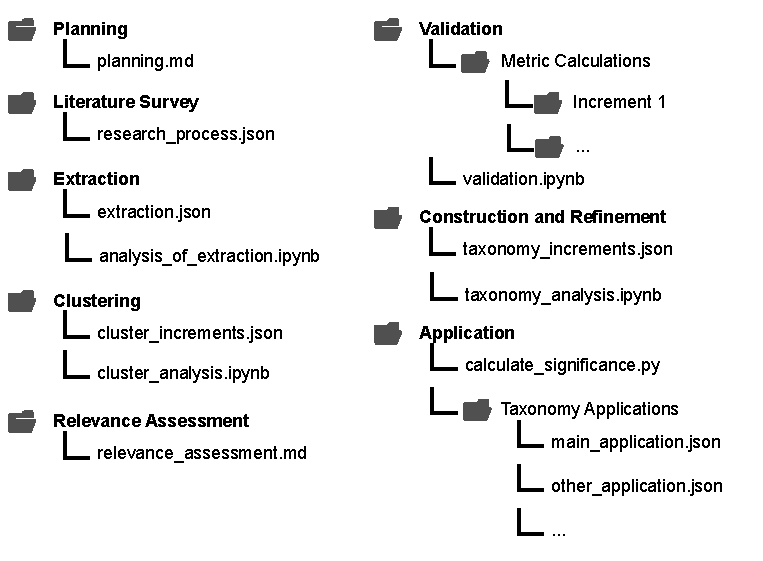
\includegraphics[width=0.7\linewidth]{figures/question_catalog/taxonomy-taxonomy_artifacts.drawio.pdf}
    \caption[Taxonomy Construction Artifacts]{Provided artifacts to support the taxonomy construction.}
    \label{fig:taxonomy_construction_artifacts}
\end{figure}

To facilitate the practical implementation of the taxonomy construction process, we provide a set of supporting artifacts, illustrated in \autoref{fig:taxonomy_construction_artifacts}, which are available in our replication package \cite{schneider_replication_2025}.

The provided artifacts are organized according to the corresponding phases of the construction process. For each phase, practitioners can access structured JSON files and Jupyter Notebooks that enable systematic execution of the process steps, comprehensive analysis of results, and calculation of relevant metrics. In addition, a usage guide is included in the replication package, offering instructions for leveraging these artifacts effectively throughout the taxonomy construction and evaluation workflow.